

\title{二维泊松方程的稳态解与加密网格方法}
\author{汤轶文 231503031}
\date{\today}

\begin{document}

\maketitle

\begin{abstract}
    本文介绍了二维泊松方程稳态解的数值求解方法。首先,推导了一维高斯热源的稳态解 \( T(r) \propto \frac{1}{r} \),并通过数值积分求解该温度场。接着,提出了加密网格方法,在热源附近增加网格分辨率以提高计算精度。最后,通过Python代码实现了该方法,并展示了温度场的可视化效果。
    \end{abstract}
    
    \section{引言}
    在热传导问题中,泊松方程描述了温度场的演化。二维泊松方程的稳态解在许多物理问题中都有广泛应用。本文通过数值积分的方法求解一维高斯热源的稳态解,并采用自适应网格细化技术来提高计算精度。
    
    \section{二维泊松方程稳态解}
    二维泊松方程的形式为:
    \[
    \nabla^2 T(x, y) = -\frac{q(x, y)}{k}
    \]
    其中,\( T(x, y) \) 是温度场,\( q(x, y) \) 是热源分布,\( k \) 是热导率。对于一个二维点热源 \( q(x, y) = \delta(x - x_0, y - y_0) \)(在 \( (x_0, y_0) \) 处),稳态解是由拉普拉斯方程的解得到的。点热源的稳态解可以写成:
    \[
    T(r) \propto \frac{1}{r}
    \]
    其中,\( r = \sqrt{(x - x_0)^2 + (y - y_0)^2} \) 是到热源的距离。
    
    对于连续的一维高斯热源,我们可以通过积分来求解温度场。热源分布为:
    \[
    q(x, y) = \frac{q_0 e^{-(x - x_0)^2 / 2\sigma^2}}{2\pi \sigma^2}
    \]
    通过积分得到的温度场为:
    \[
    T(x_0, y_0) = \int_{-\infty}^{\infty} \frac{q(x)}{\sqrt{(x - x_0)^2 + y_0^2}} dx
    \]
    该积分没有解析解,因此我们通过数值积分方法来计算该温度场。
    
    \section{数值方法:有限差分法与梯形积分}
    为了求解一维高斯热源的温度场,我们使用梯形法进行数值积分。对于每个点 \( (x_0, y_0) \),我们对 \( x \) 进行积分,得到其温度贡献。具体的数值积分公式为:
    \[
    T(x_0, y_0) \approx \sum_{i=1}^{N-1} \frac{q(x_i)}{\sqrt{(x_i - x_0)^2 + y_0^2}} \Delta x
    \]
    其中,\( x_i \) 是积分点,\( \Delta x \) 是步长。

\section{加密网格方法}
在某些物理问题中,源项可能集中在某些区域(例如热源),在这些区域我们希望获得更高的计算精度。为此,我们可以采用自适应网格细化(AMR)方法,通过动态调整网格密度来在关键区域使用更小的步长。

我们定义一个加密网格函数,该函数根据与热源的距离来调整网格的步长:
\[
h(x) = \frac{1}{1 + \frac{|x - x_0|}{A}}
\]
其中,\( x_0 \) 是热源的位置,\( A \) 是热源的扩展尺度。根据与热源的距离,步长 \( h(x) \) 会变小,从而实现加密网格。

\section{数值实验与代码实现}
为了演示加密网格方法的应用,我们考虑一个一维高斯热源,并计算其在二维空间中的温度分布。我们通过梯形法进行数值积分,并使用加密网格技术提高热源附近的计算精度。

以下是相应的Python代码实现:

\begin{verbatim}
import numpy as np
import matplotlib.pyplot as plt

def f(x, x0, y0):
    return np.exp(-x**2) / np.sqrt((x - x0)**2 + y0**2)

def refinement_function(x, x0, A):
    return 1.0 / (1 + np.exp(abs(x - x0) / A))

# 参数
N = 101
A = 1.0
x_vals = np.linspace(-A, A, N)
h = x_vals[1] - x_vals[0]

# 网格设置
xaxis = np.linspace(-5, 5, 50)
yaxis = np.linspace(-5, 5, 50)
field = np.zeros((len(xaxis), len(yaxis)))  

# 计算温度场
for i, x0 in enumerate(xaxis):
    for j, y0 in enumerate(yaxis):
        integral = 0.0
        for k in range(N - 1):
            h_adjusted = refinement_function(x_vals[k], x0, A) * (x_vals[k+1] - x_vals[k])
            integral += 0.5 * (f(x_vals[k], x0, y0) + f(x_vals[k+1], x0, y0)) * h_adjusted
        field[i, j] = integral

extent = [-5, 5, -5, 5]

fig, ax = plt.subplots(figsize=(10, 5))
c = ax.imshow(field.T, extent=extent, origin="lower", cmap="rainbow", aspect="auto")
levels = np.linspace(0, np.max(field), 20)
cs = ax.contour(xaxis, yaxis, field.T, levels, linewidths=1.5, cmap="inferno", alpha=0.5)
fig.colorbar(c, ax=ax)

ax.set_title("Contour and Color Map of Temperature Field")
ax.set_xlabel("X")
ax.set_ylabel("Y")

plt.tight_layout()
plt.show()
\end{verbatim}

\section{结果与讨论}
在图1中,我们展示了加密网格方法的应用结果。在热源附近,我们使用了较小的网格步长,从而获得了更精确的温度分布。而在远离热源的区域,使用了较大的网格步长,从而节省了计算资源。通过结合等高线图和颜色图,能够清晰地观察到温度分布的细节。

\begin{figure}[h!]
    \centering
    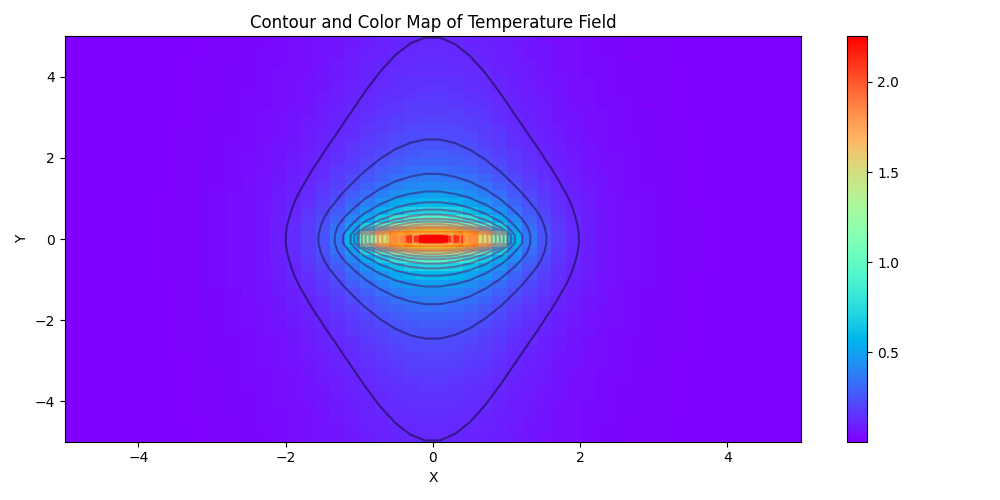
\includegraphics[width=0.8\textwidth]{temperature.png}
    \caption{加密网格法下的温度场分布,图中展示了等高线和颜色图。}
    \label{fig:temperature_field}
\end{figure}

\section{结论}
本文介绍了二维泊松方程的稳态解,并提出了加密网格方法来提高数值计算精度。通过在热源附近加密网格,能够有效提高计算精度,特别是在温度梯度变化较大的区域。我们通过数值实验和可视化展示了该方法的应用效果。

\end{document}